\begin{frame}[fragile]

  \frametitle{Adaptive MPI}

  \begin{itemize}
    \item MPI implemented on top of Charm++ 
    \item Each MPI process implemented as a user-level thread embedded in a
    chare
    \item Overdecompose to obtain communication-computation overlap between
    threads
    \item Supports migration, load balancing, fault tolerance and other Charm++
    functionality
    \item Use cases - Rocstar, BRAMS, NPB, Lulesh etc
    \item Build with AMPI as target and compile using ampi* compilers
  \end{itemize}
\end{frame}

\begin{frame}[fragile]

  \frametitle{Charm++-MPI Interoperability}

  \begin{itemize}
    \item Any library written in Charm++ can be called from MPI
    \pause
    \item Charm++ resides in the same memory space as the MPI program
    \item Control transfer between MPI and Charm++ analogous to the control transfer
    between a program and an external library being used by the program
    \pause
    \item Currently requires mpi-based build of Charm++

  \end{itemize}
\end{frame}

\begin{frame}[fragile]
  \frametitle{Interoperability Modes}
    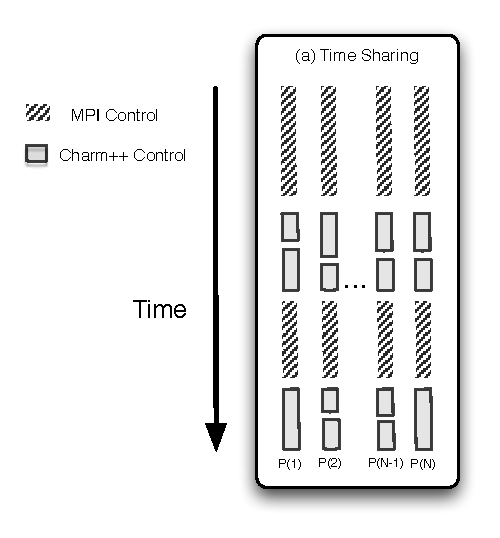
\includegraphics[width=0.45\textwidth,height=8cm]{figures/newInterop_a}
    \pause
    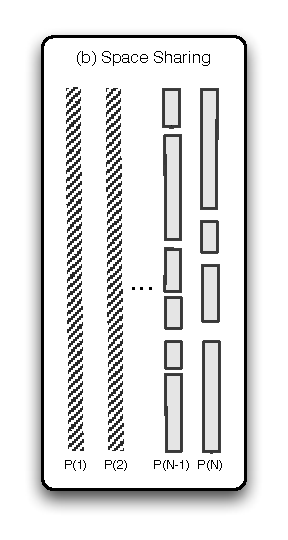
\includegraphics[width=0.275\textwidth,height=8cm]{figures/newInterop_b}
    \pause
    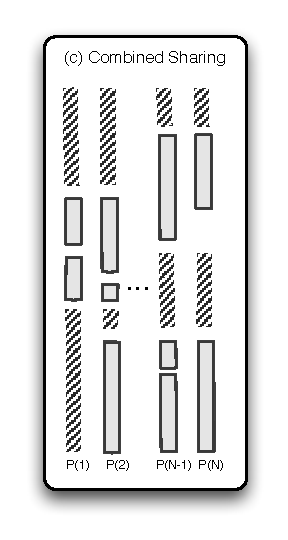
\includegraphics[width=0.275\textwidth,height=8cm]{figures/newInterop_c}
\end{frame}

\begin{frame}[fragile]
  \frametitle{Example Code Flow}
  \begin{lstlisting}[basicstyle=\footnotesize]
  MPI_Init(argc,argv); //initialize MPI
  //Do MPI related work here
  \end{lstlisting}
  \pause
  \begin{lstlisting}[basicstyle=\footnotesize]
  //create comm to be used by Charm++
  MPI_Comm_split(MPI_COMM_WORLD, myRank % 2, myRank, newComm); 
  CharmLibInit(newComm,….) //initialize Charm++ over my communicator
  \end{lstlisting}
  \pause
  \begin{lstlisting}[basicstyle=\footnotesize]
  if(myRank % 2) 
    StartHello(…); //invoke Charm++ library on one set
  else 
    //do MPI work on other set
  \end{lstlisting}
  \pause
  \begin{lstlisting}[basicstyle=\footnotesize]
  kNeighbor(…);  //invoke Charm++ library on both sets
  CharmLibExit();  //destroy Charm++ 
  \end{lstlisting}
\end{frame}

\begin{frame}[fragile]

  \frametitle{Enabling Interoperability}

  \begin{itemize}
    \item Add interface functions that can be called from MPI, and triggers
    Charm++ RTS-
    \begin{lstlisting}[basicstyle=\footnotesize]
    void HelloStart(int elems)
      if(CkMyPe() == 0) {
        CProxy_MainHello mainhello =
        CProxy_MainHello::ckNew(elems); 
      }
      StartCharmScheduler();
    }
    \end{lstlisting}
  \pause
  \item Use CkExit to return the control back to MPI
  \item Include {\em mpi-interoperate.h} in MPI and Charm++ code
  \end{itemize}
\end{frame}



